\part{User Environment}
\frame{\partpage}

{
\section{User Environment: Shell}
\usebackgroundtemplate{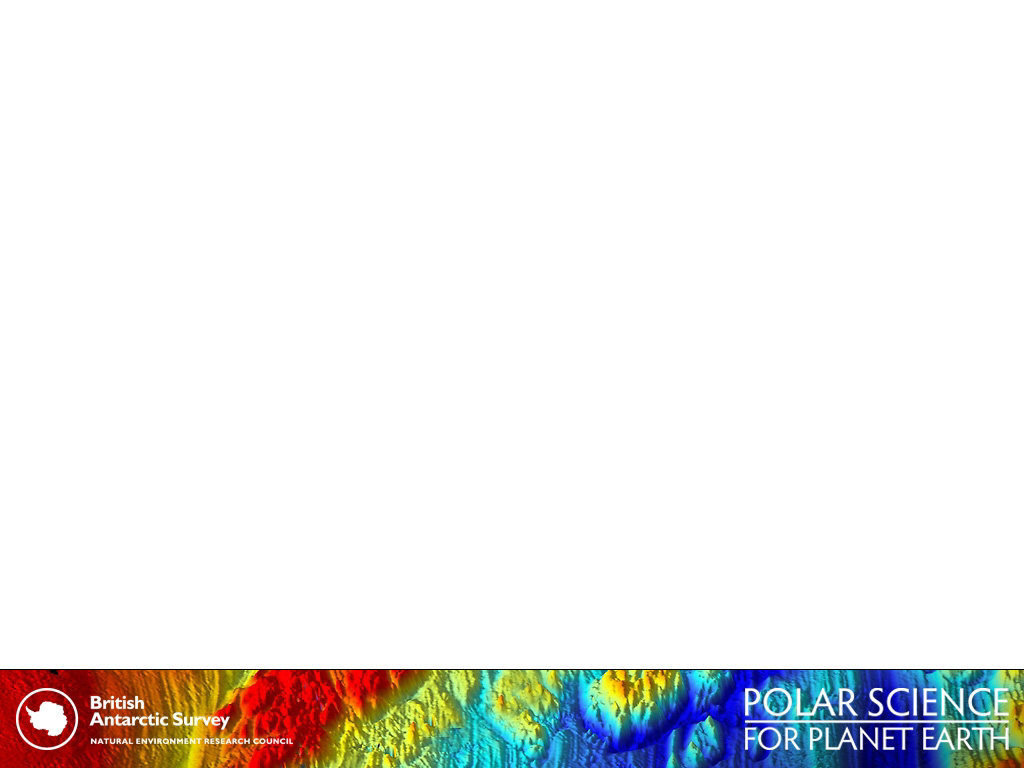
\includegraphics[width=\paperwidth]{footer_1}}%
\begin{frame}{User Environment}
\text Shell
\begin{itemize}
\item Shell
\item Our default shell is tcsh
\item If you prefer something different such as bash, contact the service desk
\end{itemize}
\end{frame}
}

{
\section{User Environment: SSH keys}
\usebackgroundtemplate{
\includegraphics[width=\paperwidth]{footer_2}}%
\begin{frame}{SSH Keys}
\begin{itemize}
\item SSH keys
\item Connect to BAS systems without typing passwords
\item ssh-keygen – Always create with a passphrase
\item ssh-agent
\item ./ssh/config
\item More information: \href{http://ictdocs/wiki/index.php/SSH\_Keys}{http://ictdocs/wiki/index.php/SSH_Keys}  
\end{itemize}
\item{{\color{red}Demonstration}}
\end{frame}
}

{
\section{User Environment: TMUX}
\usebackgroundtemplate{
\includegraphics[width=\paperwidth]{footer_3}}%
\begin{frame}{TMUX}
\begin{itemize}
\item Keeps long running command line sessions running
\item Allows disconnecting and reconnecting
\item Multiple command line sessions and console splitting
\item More information: \href{http://ictdocs/wiki/index.php/tmux}{http://ictdocs/wiki/index.php/tmux}
\end{itemize}
\item{{\color{red}Demonstration}}
\end{frame}
}

{
\section{User Environment: Software}
\usebackgroundtemplate{
\includegraphics[width=\paperwidth]{footer_4}}%
\begin{frame}{System Software}
\begin{itemize}
\item Typical linux commands and some graphical packages are installed as part of OS.
\item These can be run from the command line and desktop interface
\end{itemize}
\end{frame}
}

{
\section{User Environment: Modules}
\usebackgroundtemplate{
\includegraphics[width=\paperwidth]{footer_5}}%
\begin{frame}{The Module System}
\begin{itemize}
\item Do not work on bslcenb or bslcenc
\item There are two module repositories: /packages/modules & /hpcpackages/modules
\item Prefer /hpcpackages/modules - works with nodes and workstations
\item Modules sometimes include the compiler used in their name eg. hpc/netcdf/intel/4.4.1.1
\item Works by adjusting shell variables eg. PATH, LD_LIBRARY_PATH
\item Loaded modules only affect the terminal your loaded them in
\end{itemize}
\end{frame}
}

{
\section{User Environment: Modules (cont)}
\usebackgroundtemplate{
\includegraphics[width=\paperwidth]{footer_5}}%
\begin{frame}{Modules: useful commands}
\begin{multicols}{2}
\begin{itemize}
\item module avail 
\item module load name/version 
\item module unload name/version 

\columnbreak

\item module display name/version
\item module list
\item module purge
\end{itemize}
\end{multicols}
\end{frame}
}

{
\section{User Environment: Modules (common mistakes}
\usebackgroundtemplate{
\includegraphics[width=\paperwidth]{footer_6}}%
\begin{frame}{Common mistakes}
\begin{itemize}
\item Forgetting to use hpc modules on nodes
\item Mixing modules created using different compilers
\item Loading clashing modules
\item More information: \href{http://ictdocs/wiki/index.php?title=HPC:User_Guide}{http://ictdocs/wiki/index.php?title=HPC:User_Guide}
\end{itemize}
\item{{\color{red}Demonstration}}
\end{frame}
}

{
\section{User Environment: Modules (Jupyter Notebooks}
\usebackgroundtemplate{
\includegraphics[width=\paperwidth]{footer_7}}%
\begin{frame}{Jupyter Notebooks}
\begin{itemize}
\item Jupter notebooks running on workstations: \href{http://jupyterhub.nerc-bas.ac.uk}{http://jupyterhub.nerc-bas.ac.uk}
\item More information: \href{http://ictdocs/wiki/index.php/HPC:JupyterHub}{http://ictdocs/wiki/index.php/HPC:JupyterHub}
\end{itemize}
\end{frame}
}

{
\section{User Environment: Containers}
\usebackgroundtemplate{
\includegraphics[width=\paperwidth]{footer_8}}%
\begin{frame}{Containers}
\text Containers at BAS are still a work in progress
\begin{itemize}
\item What are containers?
\end{itemize}
\text Podman
\begin{itemize}
\item To be able to use, you need to contact the service desk
\item Container images must be downloaded to each node or workstation
\end{itemize}
\end{frame}
}

{
\section{User Environment: Containers (cont)}
\usebackgroundtemplate{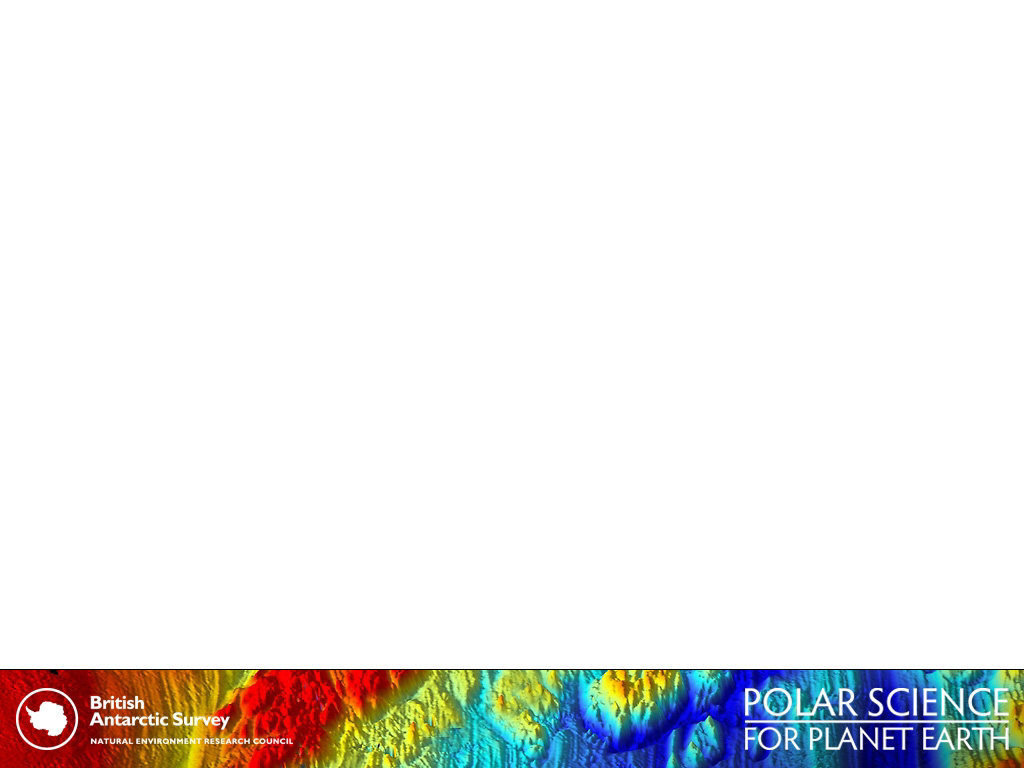
\includegraphics[width=\paperwidth]{footer_1}}%
\begin{frame}{Containers (cont)}
\text Singularity
\begin{itemize}
\item Designed with HPC usage in mind
\item Ready to use on workstations and nodes
\item For more information: \href{http://ictdocs/wiki/index.php/HPC:Containers}{http://ictdocs/wiki/index.php/HPC:Containers}
\item{{\color{red}Demonstration}}
\end{itemize}
\end{frame}
}